\documentclass{llncs}
\usepackage{graphicx}
\usepackage{float}

%%%%%%%%%%%%%%%%%%%%%%%%%%%%%%%%%%%%%%%%%%%%%%%%%%%%%%%%%%%%%%%%%%%%%%%%%%%%%

%% Options for package float
\floatstyle{ruled}
\floatname{algorithm}{Algorithm}
\newfloat{algorithm}{t}{}

%% Our own commands
\newcommand{\ignore}[1]{}
\newcommand{\textR}{\raisebox{.6ex}{\scriptsize \textregistered}}

%%%%%%%%%%%%%%%%%%%%%%%%%%%%%%%%%%%%%%%%%%%%%%%%%%%%%%%%%%%%%%%%%%%%%%%%%%%

\title{Improving the Layout of Oligonucleotide Microarrays: Pivot Partitioning}
\titlerunning{Improving Microarray Layout: Pivot Partitioning}

\author{S\'ergio A. de Carvalho Jr.\inst{1,}\inst{2}\inst{,3} \and Sven Rahmann\inst{1,}\inst{3}}
\authorrunning{S.~A.~de Carvalho Jr.~and S.~Rahmann}
\tocauthor{Sergio A.~de Carvalho Jr.\ (Universit\"{a}t Bielefeld),
Sven Rahmann (Universit\"{a}t Bielefeld)}

\institute{
International NRW Graduate School in Bioinformatics and Genome Research
\and
Graduiertenkolleg Bioinformatik, Bielefeld University, Germany \\
\email{Sergio.Carvalho@cebitec.uni-bielefeld.de}
\and
Algorithms and Statistics for Systems Biology group, Genome Informatics,
Technische Fakult\"at, Bielefeld University, D-33594 Bielefeld, Germany \\
\email{Sven.Rahmann@cebitec.uni-bielefeld.de}
}

%%%%%%%%%%%%%%%%%%%%%%%%%%%%%%%%%%%%%%%%%%%%%%%%%%%%%%%%%%%%%%%%%%%%%%%%%%%

\begin{document}

\maketitle

\begin{abstract}
The production of commercial DNA microarrays is based on a
light-directed chemical synthesis driven by a set of masks or
micromirror arrays. Because of the natural properties of light and the
ever shrinking feature sizes, the arrangement of the probes on the
chip and the order in which their nucleotides are synthesized play an
important role on the quality of the final product. We propose a new
model called \emph{conflict index} for evaluating the layout of microarrays.
We also present a new partitioning algorithm, called Pivot Partitioning,
that improves the quality of layouts, according to existing
measures, by over 6\% when compared to the best known algorithms.
\end{abstract}

%%%%%%%%%%%%%%%%%%%%%%%%%%%%%%%%%%%%%%%%%%%%%%%%%%%%%%%%%%%%%%%%%%

\section{Introduction}
\label{sec:intro}

An oligonucleotide microarray is a piece of glass or plastic on which
single-stranded fragments of DNA, called \emph{probes}, are affixed or
synthesized. Affymetrix GeneChip\textR\ arrays, for instance, can contain more
than one million spots as small as 11 $\mu$m, with each spot accommodating
several million copies of a probe. Probes are typically 25 nucleotides long
and are synthesized on the chip, in parallel, in a series of repetitive steps.
Each step appends the same nucleotide to probes of selected regions of the
chip. Selection occurs by exposure to light with the help of a
photolithographic mask that allows or obstructs the passage of light
accordingly \cite{FODOR91}.

Formally, we have a set of probes $\mathcal{P} = \{p_{1}, p_{2}, ... p_{n}\}$
that are produced by a series of masks $\mathcal{M} = (m_{1}, m_{2}, ...
m_{\mu})$, where each mask $m_{k}$ induces the addition of a particular
nucleotide $t_{k} \in \{A, C, G, T\}$ to a subset of~$\mathcal{P}$. The
\emph{nucleotide deposition sequence} $\mathcal{S} = t_{1} t_{2} \ldots
t_{\mu}$ corresponding to the sequence of nucleotides added at each masking
step is therefore a supersequence of all $p_{i} \in \mathcal{P}$
\cite{RAHMANN03}.

In general, a probe can be \emph{embedded} within $\mathcal{S}$ in several
ways. An embedding of $p_{i}$ is a $\mu$-tuple
$\varepsilon_{i} = (e_{i,1}, e_{i,2}, ... e_{i,\mu})$ in which $e_{i,k} = 1$
if probe $p_{i}$ receives nucleotide $t_{k}$ (at step~$k$), or 0 otherwise
(Fig.~\ref{fig:masking_process}). In particular, a \emph{left-most embedding}
is an embedding in which the bases are synthesized as early as possible
(see $\varepsilon_3$ in Fig.\,\ref{fig:masking_process}).

\begin{figure}
\centerline{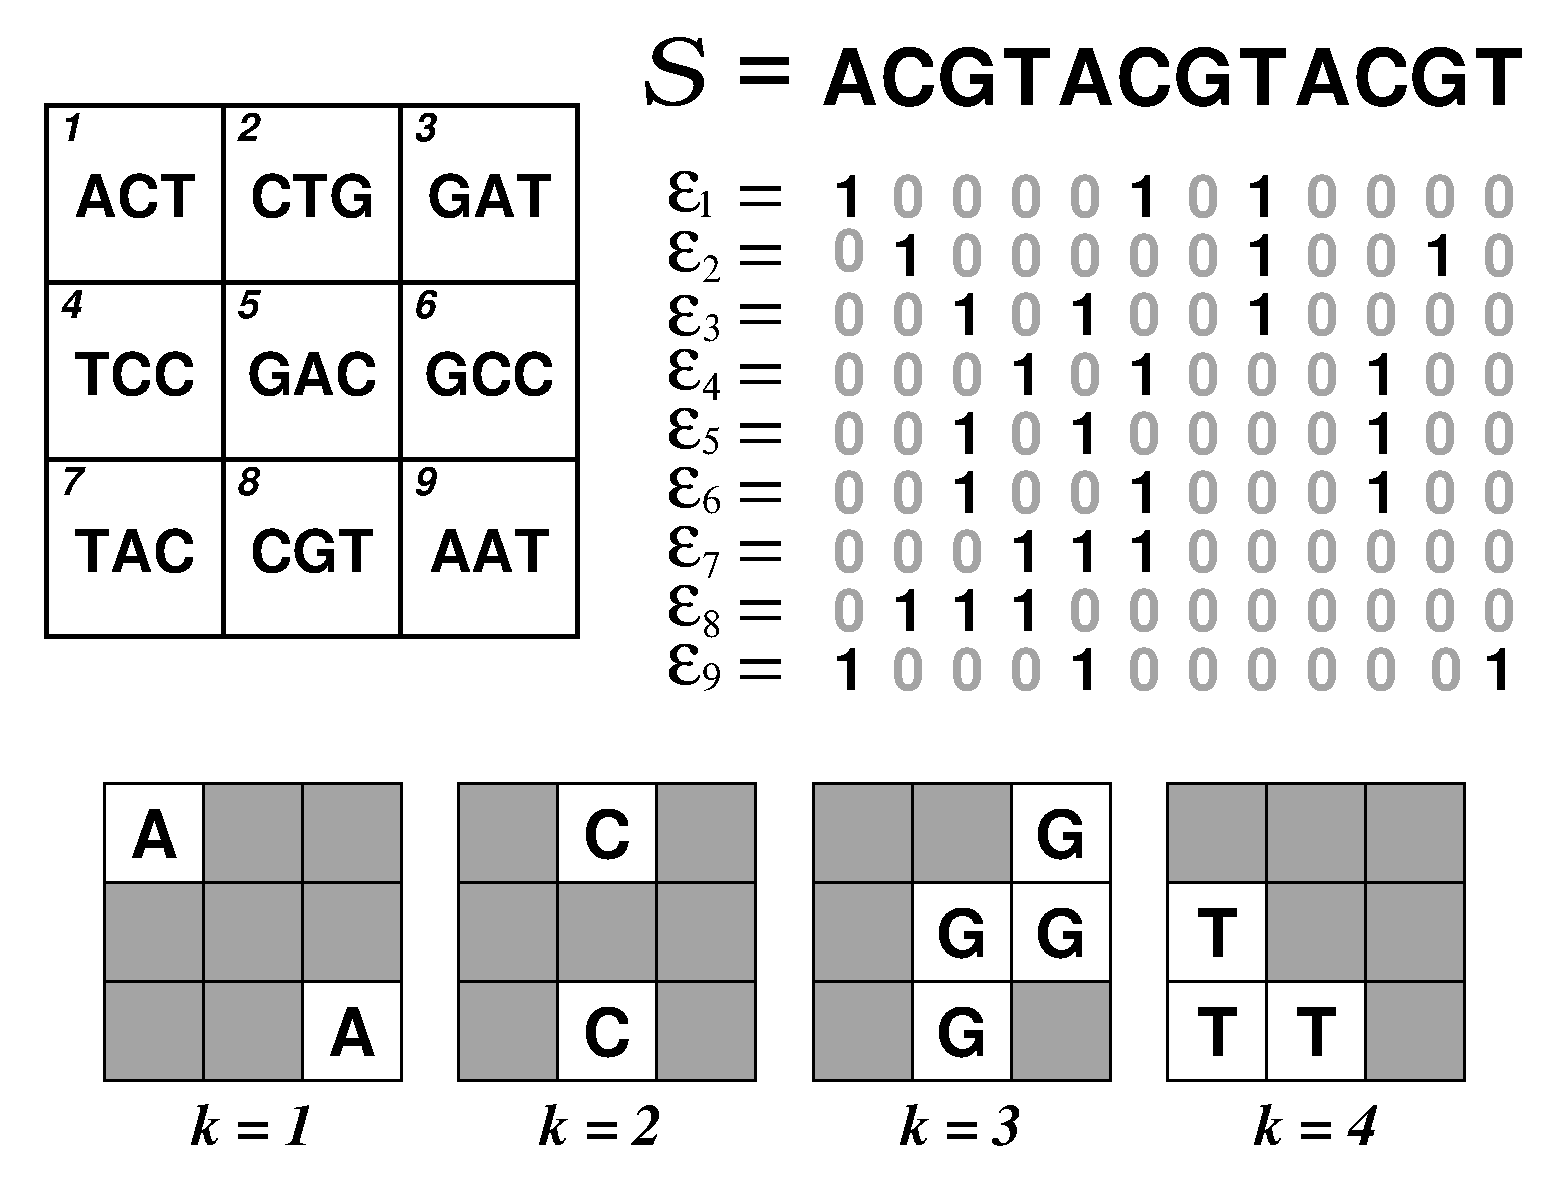
\includegraphics[width=230pt]{chip}}
\caption{Synthesis of a hypothetical 3$\times$3 chip. Top left: chip
layout and the 3~nt probe sequences. Top right: deposition
sequence and probe embeddings. Bottom: first four resulting masks.}
\label{fig:masking_process}
\vspace*{-2ex}
\end{figure}

The deposition sequence is often taken as a repeated permutation of the
alphabet, mainly because of its regular structure and because such sequences
maximize the number of distinct subsequences \cite{CHASE76}.  

We distinguish between \emph{synchronous} and \emph{asynchronous} embeddings.
In the first case, each probe has exactly one nucleotide synthesized in every
cycle of the deposition sequence; hence, 25 cycles or 100 steps are needed to
synthesize probes of length 25.  In the case of asynchronous embeddings,
probes can have any number of nucleotides synthesized in any given cycle,
allowing shorter deposition sequences. All Affymetrix chips that we know of
can be asynchronously synthesized in 74 steps (18.5 cycles), which is probably
due to careful probe selection.

Because of diffraction of light or internal reflection, untargeted spots can
be accidentally activated in a certain masking step, producing unpredicted
probes that can compromise experimental results. This problem is more likely
to occur near the borders between masked and unmasked spots~\cite{FODOR91}.
This observation has given rise to the term \emph{border conflict}.


We are interested in finding an \emph{arrangement} of the probes on the chip
together with \emph{embeddings} in such a way that the chances of unintended
illumination during mask exposure steps are minimized. The problem appears to
be hard because of the exponential number of possible arrangements, although
we are not aware of an NP-hardness proof.  In a separate
work~\cite{CARVALHO06}, we presented a formulation of the above problem as a
quadratic assignment problem (QAP), a classical combinatorial optimization
problem that is, in general, NP-hard and particularly hard to solve in
practice \cite{CELA98}. Optimal solutions are thus unlikely to be found even
for small chips and even if we assume that all probes have a single predefined
embedding. If we consider all possible embeddings (up to several million for a
typical Affymetrix probe), the problem is even harder.


For this reason, the problem has been traditionally tackled in two phases.
First, an initial embedding of the probes is fixed and an arrangement of these
embeddings on the chip with minimum border conflicts is sought. This is
usually referred to as the \emph{placement}. Second, a \emph{post-placement}
optimization phase re-embeds the probes considering its location on the chip,
in such a way that the conflicts with the neighboring spots are further
reduced.

It seems intuitive that better results should be achieved if the placement and
embedding phases are considered together, not separately. Because of the
generally high number of embeddings of each single probe in the asynchronous
setting, it is not easy to design algorithms that make efficient use of this
additional freedom and achieve reasonable running times in practice. In fact,
so far we know of no single publication that merges the two phases; in this
article we propose such a strategy called \emph{pivot partitioning}.

The rest of this paper is structured as follows. Section~\ref{sec:eval}
details two different ways of evaluating computed layouts and embeddings; they
form the objective functions that we aim to minimize. As a refinement of the
``classical'' border length of photolithographic masks, we introduce the
\emph{conflict index} measure. Section~\ref{sec:previous_work} reviews
existing placement, partitioning, and post-placement strategies.  In
Section~\ref{sec:ospe} we discuss a new variant of an optimal single probe
embedding (OSPE) algorithm that first appeared in~\cite{KAHNG02}. Our
partitioning strategy that for the first time combines partitioning the chip
with embedding the probes, is described in Section~\ref{sec:pivotpart}, and
computational results follow in Section~\ref{sec:results}.


%%%%%%%%%%%%%%%%%%%%%%%%%%%%%%%%%%%%%%%%%%%%%%%%%%%%%%%%%%%%%%%%%%%%%%%%%

\section{Evaluating Layouts and Embeddings}
\label{sec:eval}

\paragraph{Border length.}
Hannenhalli and co-workers \cite{HANNENHALLI02} were the first to give a
formal definition of the problem of unintended illumination in the production
of microarrays. They formulated the \emph{Border Length Minimization Problem}
which aims at finding an arrangement of the probes together with their
embeddings in such a way that the number of border conflicts during mask
exposure steps is minimal.

The \emph{border length}~$\mathcal{B}_k$ of a mask~$m_{k}$ is defined as the
number of borders shared by masked and unmasked spots at masking step~$k$. The
total border length of a given arrangement is the sum of border lengths over
all masks. For example, the initial four masks shown in
Fig.\,\ref{fig:masking_process} have $\mathcal{B}_1 = 4$, $\mathcal{B}_2 = 6$,
$\mathcal{B}_3 = 6$ and $\mathcal{B}_4 = 4$.  The total border length of that
arrangement is 50.



\paragraph{Conflict Index.}
The border length of an individual mask measures the quality of that
mask. We are more interested in estimating the risk of synthesizing a faulty
probe at a given spot, that is, we need a per-spot measure
instead of a per-mask measure. Additionally \cite{KAHNG03A},
the definition of border length does not take into account two
simple yet important practical considerations:
\begin{itemize}
\item[a)] stray light might activate not only adjacent neighbors but
  also probes that lie as far as three cells away from the targeted
  spot;
\item[b)] imperfections produced in the middle of a probe are more
  harmful than in its extremities.
\end{itemize}
This motivates the following definition of the \emph{conflict
  index}~$\mathcal{C}(s)$ of a spot~$s$ whose probe of
length~$\ell_{s}$ is synthesized in $\mu$~masking steps. First, we
define a distance-dependent weighting function, $\delta(s,s',k)$, that
accounts for observation a) above:
%%
\begin{equation}
\label{eq:dist_weight}
\delta(s,s',k) :=
        \left\{
                \begin{array}{ll}
                        (d(s,s'))^{-2} & \mbox{if $s'$ is unmasked at step $k$}, \\
                        0 & \mbox{otherwise}, \\
                \end{array}
        \right.
\end{equation}
%%
where $d(s,s')$ is the Euclidean distance between spots~$s$ and~$s'$.
This form of weighting function is the same as suggested in
\cite{KAHNG03A}.  Note that $\delta$ is a ``closeness'' measure
between $s$ and $s'$ only if $s'$ is
not masked (and thus creates the potential of illumination at $s$). To
limit the number of neighbors that need to be considered, we
restrict the support of $\delta(s,s',\cdot)$ to those $s'\neq s$ that
are in a $7\times 7$ grid centered around $s$ (see
Fig.\,\ref{fig:conflictindex}~left).


We also define position-dependent weights to account for observation b):
%%
\begin{equation}\label{eq:pos_mult}
\omega(s,k) :=
\left\{
  \begin{array}{ll}
    c \cdot \exp{\left(\theta \cdot \lambda(s,k)\right)} & \mbox{if $s$ is masked at step $k$}, \\
    0 & \mbox{otherwise}, \\
  \end{array}
\right.
\end{equation}
%%
where $c>0$ and $\theta>0$ are constants, and
%%
\begin{equation}\label{eq:base_pos}
  \lambda(s,k) := 1 + \min(b_{s,k},\ell_{s} - b_{s,k})
\end{equation}
%%
is the distance, from the start or end of the final probe sequence, of the
last base synthesized before step $k$: $b_{s,k}$ denotes the number of
nucleotides synthesized at spot~$s$ up to and including step~$k$, and
$\ell_s$ is the probe length (see Fig.\,\ref{fig:conflictindex}
right).

The motivation behind an exponentially increasing weighting function is that
the probability of a successful stable hybridization of a probe with its
target should increase exponentially with the absolute value of its Gibbs free
energy, which increases linearly with the length of the longest perfect match
between probe and target. The parameter $\theta$ controls how steeply the
exponential weighting function rises towards the middle of the probe.
%
\ignore{It is generally agreed that the chances of a successful hybridization
  between probe and target are higher if a mismatched base occurs at the
  extremities of the formed duplex instead of at its center. The precise
  effects of this position, however, is not yet fully understood and has been
  an active topic of research \cite{BINDER05}.}
%
In our experiments, we set $\theta := 5/\ell_s$ and $c = 1/\exp{\theta}$.


We define the conflict index of a spot $s$ as
\begin{equation}
\label{eq:conf_idx}
\mathcal{C}(s) := \sum_{k=1}^{\mu} \left( \omega(s,k) \sum_{s'} \delta(s,s',k) \right),
\end{equation}
%%
where $s'$ ranges over all spots that are at most three cells away
from $s$.  $\mathcal{C}(s)$ can be interpreted as the fraction of
faulty probes produced at spot $s$ (because of unwanted illumination).

\begin{figure}
\centerline{
%%
\begin{picture}(160,105)
\put(0,23){\makebox(160,80){
\begin{minipage}{160pt}
\centerline{\footnotesize{
\begin{tabular}{|c|c|c|c|c|c|c|c|} \hline
\ 0.06\ & \ 0.08 & \ 0.10 & \ 0.11 & \ 0.10 & \ 0.08 & \ 0.06 \\ \hline
\ 0.08\ & \ 0.13 & \ 0.20 & \ 0.25 & \ 0.20 & \ 0.13 & \ 0.08 \\ \hline
\ 0.10\ & \ 0.20 & \ 0.50 & \ 1.00 & \ 0.50 & \ 0.20 & \ 0.10 \\ \hline
\ 0.11\ & \ 0.25 & \ 1.00 &    s   & \ 1.00 & \ 0.25 & \ 0.11 \\ \hline
\ 0.10\ & \ 0.20 & \ 0.50 & \ 1.00 & \ 0.50 & \ 0.20 & \ 0.10 \\ \hline
\ 0.08\ & \ 0.13 & \ 0.20 & \ 0.25 & \ 0.20 & \ 0.13 & \ 0.08 \\ \hline
\ 0.06\ & \ 0.08 & \ 0.10 & \ 0.11 & \ 0.10 & \ 0.08 & \ 0.06 \\ \hline
\end{tabular}}}
\end{minipage}}}
\end{picture}
%%
\begin{picture}(190,105)
\footnotesize{
\put(0,0){\makebox(190,105){
  %GNUPLOT: LaTeX picture with Postscript
\begin{picture}(0,0)%
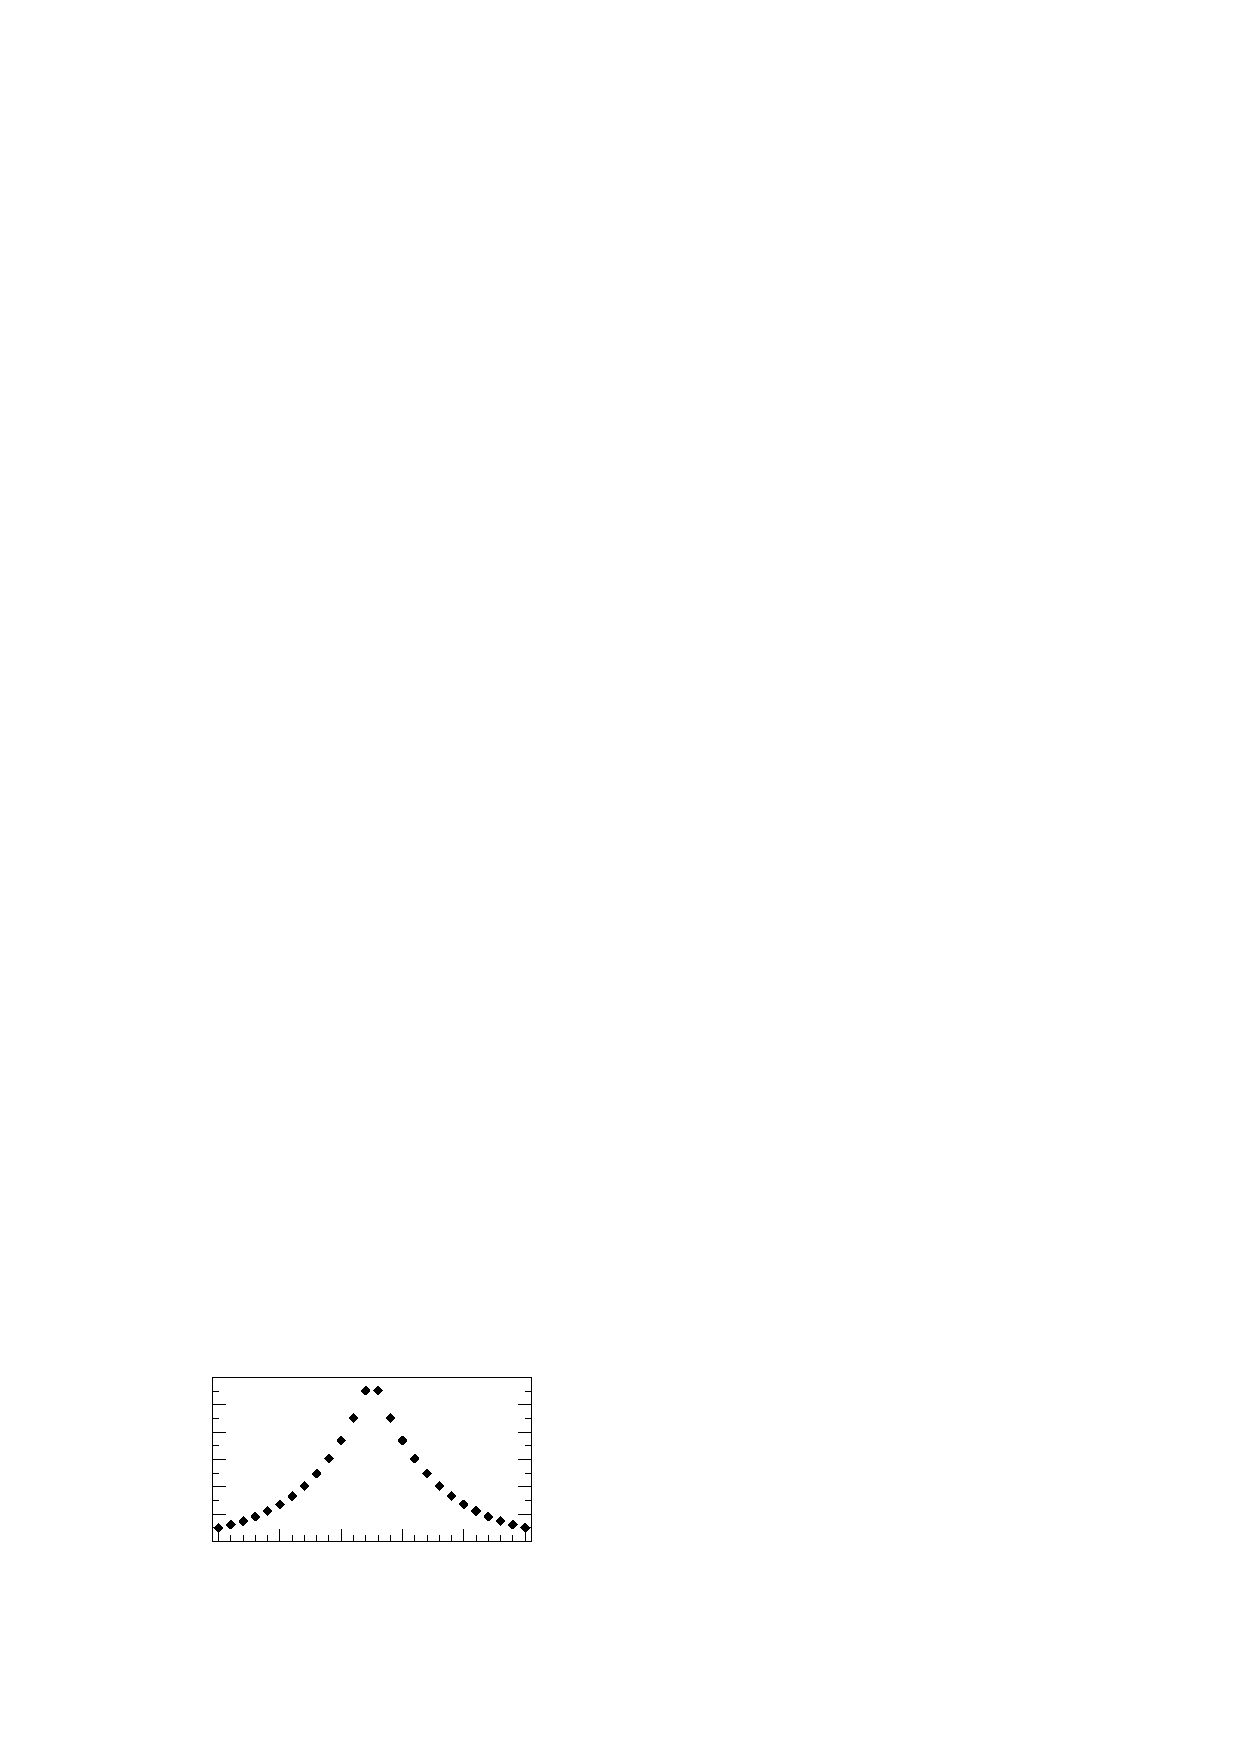
\includegraphics{position_weights}%
\end{picture}%
\begingroup
\setlength{\unitlength}{0.0200bp}%
\begin{picture}(9900,5940)(0,0)%
\put(1250,1500){\makebox(0,0)[r]{\strut{} 0}}%
\put(1250,2157){\makebox(0,0)[r]{\strut{} 2}}%
\put(1250,2813){\makebox(0,0)[r]{\strut{} 4}}%
\put(1250,3470){\makebox(0,0)[r]{\strut{} 6}}%
\put(1250,4127){\makebox(0,0)[r]{\strut{} 8}}%
\put(1250,4783){\makebox(0,0)[r]{\strut{} 10}}%
\put(1250,5440){\makebox(0,0)[r]{\strut{} 12}}%
\put(1647,1000){\makebox(0,0){\strut{} 0}}%
\put(3118,1000){\makebox(0,0){\strut{} 5}}%
\put(4589,1000){\makebox(0,0){\strut{} 10}}%
\put(6061,1000){\makebox(0,0){\strut{} 15}}%
\put(7532,1000){\makebox(0,0){\strut{} 20}}%
\put(9003,1000){\makebox(0,0){\strut{} 25}}%
\put(5325,250){\makebox(0,0){\strut{}$b_{s,k}$}}%
\end{picture}%
\endgroup
\endinput

}}}
\end{picture}
%%
}
%\vspace*{-3ex}
\caption{Ranges of values for both $\delta$ and $\omega$ on a typical 
  Affymetrix chip where probes of length~$\ell = 25$ are synthesized in $\mu =
  74$ masking steps. Left: approximate values of the distance-dependent
  weighting function $\delta(s,s',k)$ for a spot~$s$ (shown in the center) and
  close neighbors $s'$, assuming that $s'$ is unmasked at step $k$. Right:
  position-dependent weights $\omega(s,k)$ at each value of $b_{s,k}$,
  assuming that spot $s$ is masked at step $k$.}
\label{fig:conflictindex}
\end{figure}

We note the following relation between conflict indices and border lengths.
Define $\delta(s,s',k):=1$ if $s'$ is a direct neighbor of $s$ and is
unmasked in step $k$, and $:=0$ otherwise; and $\omega(s,k):=1$ if $s$ is
masked in step $k$, and $:=0$ otherwise. Then $\sum_s\, \mathcal{C}(s) = 2
\sum_{k=1}^\mu\, \mathcal{B}_k$, as each border conflict is counted twice,
once for $s$ and once for $s'$. Therefore border length and total conflict are
equivalent for a particular choice of $\delta$ and $\omega$. For our
choice~(\ref{eq:dist_weight}) and~(\ref{eq:pos_mult}), they are not
equivalent, but still correlated: A good layout has both low border length and
low average conflict index.


% ==============================================================================
\section{Previous Work}
\label{sec:previous_work}

Up to now, the tasks of probe placement and probe embedding (``post-placement
optimization'') were considered separately. Placement is often handled by
(recursively) partitioning the chip into smaller regions before applying a
placement algorithm. We now review existing placement algorithms, partitioning
algorithms and post-placement strategies.

\paragraph{Placement Algorithms.}
The border length problem on large oligonucleotide arrays of arbitrary probes
was first formally addressed in~\cite{HANNENHALLI02}. The article reports that
the first Affymetrix chips were designed using a heuristics for the traveling
salesman problem (TSP). The idea consists of building a weighted graph with
nodes representing probes, and edges containing the Hamming distance between
the probe sequences. A TSP tour is approximated, resulting in consecutive
probes in the tour being likely similar. The TSP tour is then
\emph{threaded} on the array in a row-by-row fashion.  \cite{HANNENHALLI02}
suggests a different threading of the TSP tour on the chip, called
\emph{1-threading}, to achieve up to 20\% reduction in border length.

% old version of paragraph about Epitaxial alg.
\ignore{ Kahng~{\it et~al}.~\cite{KAHNG02} propose the \emph{Epitaxial}
  placement algorithm that places a random probe in the center of the array
  and continues to insert probes in spots adjacent to already filled spots,
  employing a greedy heuristic to select the next spot to be filled and the
  probe that is assigned to it. Priority is given to spots whose neighbors are
  already filled, in which case the algorithm places the probe with minimum
  sum of Hamming distances to its neighbors. If no such a spot exists, the
  algorithm examines all non-filled spots~$s_i$ with $n_i \geq 1$ filled
  neighbors and finds a non-assigned probe $p_j$ with minimum sum of Hamming
  distances to the neighboring probes $H_{ij}$. For each possible assignment
  of $p_j$ to $s_i$, it computes a cost $c(s_i,p_j) := k_{n_i} H_{ij} / n$,
  where $k_{n_i}$ are scaling coefficients ($k_1 = 1$, $k_2 = 0.8$, and $k_3 =
  0.6$), and makes the assignment with minimum cost. With this algorithm, they
  claimed to achieve up to 10\% reduction in border conflicts over the
  TSP-based approach of Hannenhalli~{\it et~al}.\ \cite{HANNENHALLI02}.
%  
}

A different strategy called \emph{Epitaxial} placement
\cite{KAHNG02} places a random probe in the center of the array and continues
to insert probes in spots adjacent to already filled spots. Priority is given
to spots with the largest numbers of filled neighbors. At each iteraction, it
examines all non-filled spots~$s_i$ and finds a non-assigned probe $p_j$ with
minimum sum of Hamming distances $H_{ij}$ to the neighboring probes, employing
a greedy heuristic to select the next spot.  A further 10\% reduction in
border conflict over TSP\,+\,1-threading is claimed.

\ignore{
The major problem with the Epitaxial and the TSP-based algorithm is that they
have at least quadratic time complexity and thus are not scalable for the
latest million-probe microarrays. According to their experiments, the TSP
approach needed around 32 minutes to produce the layout of a 200\,x\,200
chip, whereas the Epitaxial algorithm needed 74 minutes on average. For a
500\,x\,500 chip, the TSP took over 30 hours to complete, whereas the
Epitaxial algorithm did not complete ``due to prohibitively large running
time or memory requirements'' \cite{KAHNG02}.
}

\ignore{
This observation has led to the development of two new algorithms by
\cite{KAHNG03A}. The first one, called Sliding-window Matching (SWM), is not
exactly a placement algorithm as it iteratively improves an initial placement
that can be constructed by, for instance, TSP and 1-threading. Improvements
are achieved by selecting an independent set of spots inside the window and
optimally replacing their probes using a minimum-weight perfect matching
algorithm. The term independent refers to probes that can be replaced without
affecting the border length of the other selected probes.
}

Both the Epitaxial algorithm and the TSP approach do not scale well to large
chips. For this reason, \cite{KAHNG03A} proposes a simpler variant of the
Epitaxial algorithm, called \emph{Row-epitaxial}, with two main differences:
spots are filled in a pre-defined order, namely from top to bottom, left to
right, and only probes of a limited list of candidates are considered when
filling each spot. Experiments show that Row-epitaxial is the best
large-scale placement algorithm, achieving up to 9\% reduction in border
length over the TSP\,+\,1-threading.


\paragraph{Partitioning Algorithms.}
The placement problem can be partitioned by dividing the set of probes into
smaller sub-sets, and assigning these sub-sets to sub-regions of the chip.
Each sub-region can then be treated as an independent chip or recursively
partitioned. These smaller sub-problems, when solved, immediately constitute a
final solution. In this way, algorithms with non-linear time or space
complexities can be used to compute the layout of larger chips that otherwise
would not be feasible.

The only partitioning that we know of is the Centroid-based
Quadrisection~\cite{KAHNG03B}. It starts by randomly selecting a probe
$c_1 \in \mathcal{P}$. Then, it selects another probe $c_2$ maximizing
$h(c_1,c_2)$, the Hamming distance between their embeddings. Similarly, it
selects $c_3$ and $c_4$ maximizing the sum of Hamming distance between these
four probes that are called centroids. All other probes $p_i \in \mathcal{P}$
are then compared to the centroids and assigned to the sub-set $\mathcal{P}_j$
associated with $c_j$ with minimum $h(p_i,c_j)$. The chip is divided into four
quadrants, each being assigned to a sub-set $\mathcal{P}_j$ .  The procedure
is repeated recursively on each quadrant until a given recursion depth is
reached. In the end, the Row-epitaxial algorithm is used to produce the
placement of the probes in each final sub-region.


\paragraph{Post-placement Optimization.}
Once the placement is done, further reduction of conflicts can be achieved by
re-embedding the probes without changing their locations.  The paper
\cite{KAHNG02} presents a dynamic programming algorithm, that we call Optimum
Single Probe Embedding (OSPE), for computing an optimum embedding of a probe
on a spot $s$ with respect to the probes of neighboring spots, whose
embeddings are considered fixed.  Originally, it was developed for border
length minimization; below (Sect.~\ref{sec:ospe}) we give a slightly more
general form that also applies to the conflict index measure.

The OSPE algorithm is the basic operation of several post-placement
optimization algorithms: Batched Greedy~\cite{KAHNG02},
Chessboard~\cite{KAHNG02} and Sequential~\cite{KAHNG03B}. Their main
difference lies in the order in which the re-embeddings take place.

\ignore{ The first algorithm is a simple greedy approach that computes, for
  each spot of the chip, the maximum reduction of conflicts that could be
  achieved by re-embedding its probe with the OSPE algorithm. It then greedily
  selects the spot with higher gain and re-embeds its probe optimally with
  respect to its neighbors, updating the gains of affected spots. A faster
  version, called Batched Greedy, sacrifices its greedy nature by postponing
  the update of gains and re-embedding all probes that have not been affected
  by the re-embeddings performed in the current iteration.
  
  The Chessboard optimization is based on the fact that a chip can be
  bi-colored just like a chessboard, in such a way that the embeddings of
  probes located on white spots, with respect to border length, are
  independent of those placed on black spots, and vice-versa. The Chessboard
  uses this coloring to alternate the optimal re-embedding of probes located
  on black and white spots.%
}

The Sequential algorithm is a simple but so far the most effective
post-placement optimization. It just proceeds spot by spot, from top to
bottom, left to right, re-embedding all probes with the OSPE algorithm.
Surprisingly, it achieves the greatest reduction of border conflicts with a
running time compared to the Batched Greedy, the faster among the three.

The OSPE algorithm never increases the amount of conflicts in a region.  All
optimization algorithms can thus be executed several times until a local
optimal solution is found, or until the improvements drop below a given
threshold.


%%%%%%%%%%%%%%%%%%%%%%%%%%%%%%%%%%%%%%%%%%%%%%%%%%%%%%%%%%%%%%%%%%%%%%%%%%%
\section{Optimum Single Probe Embedding}
\label{sec:ospe}

The Optimum Single Probe Embedding (OSPE) algorithm finds an optimal
embedding of a single probe on a given spot, assuming that all neighboring
embeddings are fixed. It can be seen as a special case of a global alignment
between the probe sequence $p$ of length $\ell$ and the deposition sequence
$\mathcal{S}$ of length $\mu$. We use an $(\ell + 1) \times (\mu + 1)$ array
$D$, where $D[i,j]$ is defined as the minimum cost of an embedding of
$p[1..i]$ into $\mathcal{S}[1..j]$.  The cost is the sum of conflicts induced
by the embedding of $p$ on its neighbors plus the conflicts suffered by $p$
because of the embeddings of its neighbors.

At every step $j$ of the deposition sequence, the spot $s$ can be either
masked or unmasked. Thus, entry $D[i,j]$ is computed as the minimum between
the costs resulting from each possible action:
%%
\[
D[i,j] = \min (D[i,j-1] + M_{ij}, D[i-1,j-1] + U_{j}).
\]

The costs $M_{ij}$ and $U_{j}$ depend on the spot $s$ and the neighboring
spots $s'$.
$M_{ij}$ denotes the cost of masking spot $s$ at step $j$ given that base $i$
of probe $p$ has been synthesized previously.  Any unmasked neighbor $s'$
generates a conflict on $s$ with cost $\omega(s,i)\cdot \delta(s,s',j)$;
therefore the total cost is
\[ M_{ij} = \sum_{s'}\, \omega(s,i) \cdot \delta(s,s',j). \]

$U_{j}$ denotes the cost of unmasking spot $s$ at step $j$; it generates a
conflict on each masked neighbor $s'$ with cost $\omega(s',j)\cdot
\delta(s',s,j)$; therefore 
\[ U_j = \sum_{s'}\, \omega(s',j) \cdot \delta(s',s,j). \]

The first column of $D$ is initialized as follows: $D[0,0] = 0$ and $D[i,0] =
\infty$ for $0 < i \leq \ell$. The first row is $D[0,j] = D[0,j-1]+M_{0j}$ for
$0<j\leq\mu$.
The time complexity of the OSPE algorithm is obviously $O(\ell_p \cdot
|\mathcal{S}|)$, where $\ell_p$ is the length of probe $p$ and $|\mathcal{S}|$
is the length of the deposition sequence.


% ==============================================================================
\section{Pivot Partitioning}
\label{sec:pivotpart}

Traditionally, the microarray layout problem has been tackled in two phases:
placement, during which an initial embedding of the probes is fixed, and
post-placement optimization, when probes are re-embedded using the OSPE algorithm.
We believe that better layouts can be produced if the placement phase also considers
the various embeddings that a probe can have. In this section we propose a new
partitioning algorithm called Pivot Partitioning (PP).

Our algorithm
has some similarities with the Centroid-based Quadrisection (CQ) described
in Sect.\,\ref{sec:previous_work}.
Its main differences are motivated by the following observation.
As mentioned earlier, some probes can have up to several millions different
embeddings, while others may have only a few or even only one possible embedding.
Probes with more embeddings can better
``adapt'' to the other probes, that is, when placed on a spot, they are more likely
to have an embedding with fewer conflicts than a probe that has
only a limited number of embeddings.

We use the probes with fewer embeddings, that we call ``pivots'', to drive the
partitioning of the probe set and to re-embed the probes just before their
placement (as a partitioning algorithm, PP also works in combination with
another placement algorithm). Also, we designed our algorithm to work for border
length minimization as well as conflict index minimization.

\begin{algorithm}
\caption{Pivot Partitioning}
\label{alg:pivotpart}
\begin{minipage}{4.8in}

\begin{tabbing}
Output: \=                                  \kill
Input:  \> chip dimension,                          \\
        \> set of probes $\mathcal{P} = \{p_{1}, p_{2}, ... p_{n}\}$,       \\
        \> maximum partitioning depth $t_{max}$                 \\
Output: \> placement of the probes $p \in \mathcal{P}$ on the chip
\end{tabbing}

\begin{enumerate}
\item Select probes $p$ with minimum number of embeddings, $E(p)$,
as pivot candidates:
  \begin{enumerate}
  \item Let $\mathcal{Q} = \{p \in \mathcal{P} | E(p) \mbox{ is minimal}\}$
  \item Set $\mathcal{P} \leftarrow \mathcal{P} \setminus Q$
  \end{enumerate}
\item Define a region $R$ of the chip containing all of its rows and columns
\item Call the Recursive Partitioning with the initial partitioning depth 1:
  \begin{enumerate}
  \item Return Recursive Partitioning (1, $t_{max}$, $R$, $\mathcal{Q}$, $\mathcal{P}$)
  \end{enumerate}
\end{enumerate}

\end{minipage}
\end{algorithm}

% ------------------------------------------------------------------------------
\subsection{Pivot Candidates}

The first step of the Pivot Partitioning (Algorithm\,\ref{alg:pivotpart}), is to
select the pivot candidates $\mathcal{Q}$, a set of probes that can later be
chosen as pivots. Our pivots are the equivalent of the centroids of the CQ
algorithm; they are used to partition the probe set. Their
selection, however, is restricted to the probes having fewer embeddings.

The reasons are two-fold. First, less time is spent choosing the pivots
since less candidates need to be examined.
Second, probes with fewer embeddings are better representatives to drive
the partitioning. The problem is that some embeddings may have their unmasked steps
concentrated in one region of the deposition sequence. This is specially true if
the probes are embedded in a left-most or right-most fashion.
Some Affymetrix probes, for instance,
can be synthesized in the first 37 masking steps, thus
using only half of the total 74 steps. Such probes are clearly not good choices
for pivots. Probes with fewer embeddings, on the other hand,
are guaranteed to cover most (if not all) cycles of the deposition sequence.

In order to guarantee a good partitioning,
we limit the size of $\mathcal{Q}$ to a minimum of 1\% of the total
number of probes\footnote{Usually, around 1-2\% of the probes of an Affymetrix array
have only one possible embedding; or two, if we consider that they appear in PM/MM
pairs and must be ``aligned'' in all but the steps that synthesize their middle
bases}. This is achieved by selecting probes with the next minimum
number of embeddings.
Computing the number of embeddings of a probe takes $O(\ell \mu)$ time, where
$\ell$ is the length of the probe and $\mu$ is the length of the deposition sequence.
With a few simple optimizations, however, even a million probes can be examined in
a few minutes.

% ------------------------------------------------------------------------------
\subsection{Recursive Partitioning}

\begin{algorithm}
\caption{Recursive Partitioning}
\label{alg:recursivepart}
\begin{minipage}{4.8in}

\begin{tabbing}
Output: \=                                  \kill
Input:  \> current depth level $t$,                     \\
        \> maximum depth level $t_{max}$                    \\
        \> rectangular region $R$ of the chip,                  \\
        \> set of pivot candidates $\mathcal{Q}$,               \\
        \> set of probes $\mathcal{P}$,                     \\
Output: \> placement of the probes $p \in \mathcal{P}$ and
           $q \in \mathcal{Q}$ on the region $R$ of the chip
\end{tabbing}

\begin{enumerate}
\item If $t = t_{max}$ then
  \begin{enumerate}
    \item Re-embed $p \in \mathcal{P}$ optimally with respect to all $q \in \mathcal{Q}$
    \item Return Row-epitaxial ($R$, $\mathcal{P} \cup \mathcal{Q}$)
  \end{enumerate}
\item Select $q'$ and $q'' \in \mathcal{Q}$ such that $h(q',q'')$ is maximal
\item \label{step:part_pivots} Partition the set of pivot candidates:
  \begin{enumerate}
    \item $\mathcal{Q}' = \{q \in \mathcal{Q} | h(q,q') < h(q,q'')\}$
    \item $\mathcal{Q}'' = \{q \in \mathcal{Q} | h(q,q') > h(q,q'')\}$ \\
    (when $h(q,q') = h(q,q'')$, assignments are made in an attempt to
    achieve balanced partitionings)
  \end{enumerate}
\item Partition the set of probes:
  \begin{enumerate}
    \item $\mathcal{P}' = \{p \in \mathcal{P} | w(p,q') < w(p,q'')\}$
    \item $\mathcal{P}'' = \{p \in \mathcal{P} | w(p,q') > w(p,q'')\}$ \\
    (when $h(p,q') = h(p,q'')$, assignments are made in an attempt to
    achieve balanced partitionings)
  \end{enumerate}
\item \label{step:part_r} Partition $R$ into two sub-regions proportionally to the number of probes
      in $\mathcal{P}' \cup \mathcal{Q}'$ and $\mathcal{P}'' \cup \mathcal{Q}''$
\item Return Recursive Partitioning ($t + 1$, $t_{max}$, $R'$, $\mathcal{Q}'$, $\mathcal{P}$') \\
      $\cup$ Recursive Partitioning ($t + 1$, $t_{max}$, $R''$, $\mathcal{Q}''$, $\mathcal{P}$'')
\end{enumerate}

\end{minipage}
\end{algorithm}

The essence of the Pivot Partitioning algorithm is its recursive procedure
(Algorithm\,\ref{alg:recursivepart}), that is executed until a given
recursion depth $t_{max}$ is reached.

If the maximum recursion depth has not been reached yet, we choose a pair of
pivots $q'$ and $q'' \in \mathcal{Q}$ with maximum Hamming distance
between their embeddings, $h(q',q'')$. All other $q \in \mathcal{Q}$ are
assigned to a sub-set of $\mathcal{Q}$ associated with the pivot whose
Hamming distance to $q$ is minimum (step~\ref{step:part_pivots}).

The next step similarly partitions $\mathcal{P}$ into two sub-sets. A probe
$p \in \mathcal{P}$ is assigned to the sub-set associated with the pivot $q$
with minimum weighted distance $w(p,q)$. The weighted distance is computed
with the OSPE algorithm, ignoring the location of the probes since they have
not been placed yet. In this way, we make the assignments considering all
possible embeddings of $p$.

Step \ref{step:part_r} partitions $R$ into two sub-regions, proportionally to the
number of probes in $\mathcal{Q}' \cup \mathcal{P}'$ and $\mathcal{Q}'' \cup \mathcal{P}''$.
We alternate between horizontal and vertical divisions at each partitioning depth $t$.
Since we only deal with rectangular regions, sometimes it is necessary to move
a few probes from one partition to the other in order to ensure that the probes
fit in the sub-regions.

Each sub-region is then processed recursively. Once the maximum partitioning depth
$t_{max}$ is reached, the Row-epitaxial~\cite{KAHNG03A} algorithm is
called to place the probes of $\mathcal{P} \cup \mathcal{Q}$ in the region $R$.
Before that, however, all probes $p_i \in \mathcal{P}$ are re-embedded optimally
with respect to the pivots. Again, we use the OSPE algorithm ignoring their location.
This is done to help the placement algorithm by improving the ``alignment'' of all
embeddings in the region.

% ==============================================================================
\section{Results and Discussion}
% ==============================================================================
\label{sec:results}

We now present the results of running our Pivot Partitioning (PP) algorithm on
random chips. Table~\ref{tab:pp_bl} shows the normalized border length (total border
length divided by the number of probes) using our own implementations of Row-epitaxial
(for the placement) as well as the Sequential post-placement optimization.

Our results
show that, in the first level of partitioning, PP allows for a reduction in border length
by as much as 16\% when compared to running the Row-epitaxial alone (from 41.27 to
34.69 on $500\times 500$ chips). The total border length for $t_{max}=2$ on
$500\times 500$ is 8\,673\,722. This represents a reduction of as much as 6.8\% over
the layout produced by the Centroid-based Quadrisection (CQ) similarly combined with
Row-epitaxial and followed by the Sequential optimization, which produced a layout
with a border length of 9\,307\,510 as reported in~\cite{KAHNG03B}. In the next levels
of partitioning, we observe a small increase in border length but, on the other hand,
we also report a significant reduction in running times.

Table~\ref{tab:pp_ci} shows similar results with the average conflict index. For these
experiments, we use a version of Row-epitaxial implemented for conflict index
minimization, which fills every spot $s$ with a probe minimizing $\mathcal{C}(s)$.
For the post-placement optimization,
we use the Sequential algorithm with the OSPE for conflict index minimization
as described in Sect.\,\ref{sec:ospe}. Computing the conflict index of a spot for
every probe candidate is not as straight forward as computing the Hamming distance
between a probe
and its neighbors, and thus both versions of the Row-epitaxial and the Sequential
optimization for conflict index minimization are significantly slower. For this reason,
we set the limit on the number of probes considered by the Row-epitaxial to $Q = 2\,000$.

\begin{table}[t]
\caption{
Normalized border length of layouts produced by Pivot Partitioning on random chips
with dimensions ranging from $100\times 100$ to $500\times 500$, with probes
synchronously embedded in a deposition sequence of length 100. Partitioning
depths ranges from $t_{max}=0$ (no partitioning) to $t_{max}=6$. Row-epitaxial
is used for the placement (with $Q = 20\,000$), followed by the Sequential
post-placement optimization. Running times are reported in seconds, and do not
include the post-placement optimization.}
\centerline{
\begin{tabular}{clrrlrrlrrlrr}
\label{tab:pp_bl}
& & \multicolumn{2}{c}{$t_{max}=0$} & & \multicolumn{2}{c}{$t_{max}=2$} & & \multicolumn{2}{c}{$t_{max}=4$} & & \multicolumn{2}{c}{$t_{max}=6$} \\
\noalign{\smallskip}
Dim & & \multicolumn{1}{c}{Cost} & \multicolumn{1}{c}{Time} & & \multicolumn{1}{c}{Cost} & \multicolumn{1}{c}{Time} & & \multicolumn{1}{c}{Cost} & \multicolumn{1}{c}{Time} & & \multicolumn{1}{c}{Cost} & \multicolumn{1}{c}{Time} \\
\noalign{\smallskip}
\cline{1-1} \cline{3-4} \cline{6-7} \cline{9-10} \cline{12-13}
\noalign{\smallskip}
100 & \ \ & \ 42.77 & \     34 & \ \ & \ 39.19 & \     13 & \ \ & \ 40.72 & \     10 & \ \ & \ 42.11 & \  11 \\
200 & \ \ & \ 41.63 & \    429 & \ \ & \ 37.30 & \    155 & \ \ & \ 38.53 & \     62 & \ \ & \ 40.00 & \  85 \\
300 & \ \ & \ 41.38 & \ 1\,174 & \ \ & \ 36.12 & \    766 & \ \ & \ 37.22 & \    264 & \ \ & \ 38.53 & \ 139 \\
500 & \ \ & \ 41.27 & \ 3\,524 & \ \ & \ 34.69 & \ 3\,472 & \ \ & \ 35.50 & \ 1\,996 & \ \ & \ 36.58 & \ 713 \\
\noalign{\smallskip}
\hline
\end{tabular}}
\end{table}

\begin{table}[t]
\caption{
Average conflict index of layouts produced by Pivot Partitioning on random chips
of synchronous embeddings. We use versions of the Row-epitaxial (with $Q = 2\,000$)
and the Sequential algorithms for conflict index minimization.}
\centerline{
\begin{tabular}{clrrlrrlrrlrr}
\label{tab:pp_ci}
& & \multicolumn{2}{c}{$t_{max}=0$} & & \multicolumn{2}{c}{$t_{max}=2$} & & \multicolumn{2}{c}{$t_{max}=4$} & & \multicolumn{2}{c}{$t_{max}=6$} \\
\noalign{\smallskip}
Dim & & \multicolumn{1}{c}{Cost} & \multicolumn{1}{c}{Time} & & \multicolumn{1}{c}{Cost} & \multicolumn{1}{c}{Time} & & \multicolumn{1}{c}{Cost} & \multicolumn{1}{c}{Time} & & \multicolumn{1}{c}{Cost} & \multicolumn{1}{c}{Time} \\
\noalign{\smallskip}
\cline{1-1} \cline{3-4} \cline{6-7} \cline{9-10} \cline{12-13}
\noalign{\smallskip}
100 & \ \ & \ 514.49 & \     45 & \ \ & \ 453.67 & \     37 & \ \ & \ 467.78 & \     19 & \ \ & \ 475.44 & \     15 \\
200 & \ \ & \ 517.07 & \    192 & \ \ & \ 466.22 & \    215 & \ \ & \ 452.41 & \    166 & \ \ & \ 462.55 & \     99 \\
300 & \ \ & \ 518.51 & \    438 & \ \ & \ 475.84 & \    524 & \ \ & \ 452.00 & \    466 & \ \ & \ 448.17 & \    336 \\
500 & \ \ & \ 517.50 & \ 1\,471 & \ \ & \ 481.36 & \ 1\,530 & \ \ & \ 462.33 & \ 1\,472 & \ \ & \ 445.43 & \ 1\,295 \\
\noalign{\smallskip}
\hline
\end{tabular}}
\end{table}

\ignore{
The results shown on table Table~\ref{tab:pp_x_cq_bl} are for chips with probes
synchronously embedded. For chips with asynchronous embeddings, PP is likely
to produce even better results when compared to CQ. This is because our
pivots are selected from the probes having fewer embeddings, which are likely
to be better representatives.
} %% we would have to show data on synchronous chips to state that

\begin{table}
\caption{Comparison between Pivot Partitioning (PP) and Centroid-based Quadrisection (CQ)
on random chips with dimensions ranging from $100\times 100$ to $500\times 500$, whose probes
are synchronously embedded in a deposition sequence of length 100. The partitioning
depths varies from $L=1$ to $L=3$ for the CQ algorithm and, equivalently, from
$t_{max}=2$ to $t_{max}=6$ for PP. Both partitionings use Row-epitaxial for the placement
(with $Q = 20\,000$) and are followed by the Sequential post-placement optimization.
The data shows the total border length of chips produced by CQ
(extracted from~\cite{KAHNG03B}), and the results of using PP on
similar input, as percentage of the reduction in border length compared to CQ. For
instance, PP generates on average 8.95\% less border length on $500\times 500$ chips
with $t_{max}=2$.}
\centerline{
\begin{tabular}{clrrlrrlrr}
\label{tab:pp_x_cq_bl}
& & \multicolumn{1}{c}{CQ} & \multicolumn{1}{c}{PP} & & \multicolumn{1}{c}{CQ} & \multicolumn{1}{c}{PP} & & \multicolumn{1}{c}{CQ} & \multicolumn{1}{c}{PP} \\
\noalign{\smallskip}
Dim & & \multicolumn{1}{c}{$L=1$} & \multicolumn{1}{c}{$t_{max}=2$} & & \multicolumn{1}{c}{$L=2$} & \multicolumn{1}{c}{$t_{max}=4$} & & \multicolumn{1}{c}{$L=3$} & \multicolumn{1}{c}{$t_{max}=6$} \\
\noalign{\smallskip}
\cline{1-1} \cline{3-4} \cline{6-7} \cline{9-10}
\noalign{\smallskip}
100 & & \    393\,218 & \ 0.18\% & & \    399\,312 & \ -1.89\% & & \    410\,608 & \ -2.48\% \\
200 & & \ 1\,524\,803 & \ 2.27\% & & \ 1\,545\,825 & \  0.48\% & & \ 1\,573\,096 & \ -1.34\% \\
300 & & \ 3\,493\,552 & \ 7.12\% & & \ 3\,413\,316 & \  2.05\% & & \ 3\,434\,964 & \ -0.61\% \\
500 & & \ 9\,546\,351 & \ 8.95\% & & \ 9\,355\,231 & \  4.67\% & & \ 9\,307\,510 & \  1.03\% \\
\noalign{\smallskip}
\hline
\end{tabular}}
\end{table}

\ignore{
\multicolumn{10}{c}{Results for PP are averages over five random chips uniformly generated.\\
Experiments were conducted on a Sun Fire V1280 server with 900Mhz UltraSparc III+ processors \\
and 96 Gb of RAM under similar load balances.}
}

\ignore{
Tables~\ref{tab:pp_affy_bl} and~\ref{tab:pp_affy_ci} shows the results of running PP on chips
containing probe sets of existing Affymetrix GeneChip arrays -- E.Coli 2.0 Genome (EC2), Porcine
Genome (POR) and Wheat Genome (WHT) -- whose probes are synchronously embedded in a deposition
sequence of length 74. Table~\ref{tab:pp_affy_bl} shows the normalized border length
(total border length divided by the number of probes) while Table~\ref{tab:pp_affy_ci} shows
the average conflict index.
} %% results on Affy chips

We also compare the performance of Pivot Partitioning with the
Centroid-based Quadrisection (CQ). Table~\ref{tab:pp_x_cq_bl} shows the total border
length of layouts produced by CQ as reported in ~\cite{KAHNG03B}. We run PP
on similar input and report the results with equivalent partitioning depths
(two levels of PP are equivalent to one level on CQ). The results are shown
as a percentage of reduction in border length compared to CQ. For instance,
on $500\times 500$ chips, PP produces layouts with 8.95\% less conflicts than
CQ, on average.

Our results
show that PP produces layouts with less conflicts than CQ except for higher
partitioning depths on the smaller chips. We suspect that this disadvantage is
due to the ``borrowing heuristic'' used by CQ that permits, during the placement,
borrowing probes from neighboring partitions in order to maintain a high number
of probes that can be considered for filling the last spots of a quadrant. We are
planning to investigate a similar strategy on Pivot Partitioning that could improve
the quality of our solutions.

\paragraph{Summary}
We have presented a new partitioning strategy that for the first time combines
the partitioning the chip with embedding of the probes. The main advantages of
our approach over previous methods are: faster and better selection of pivots
used to drive the assignment of probes to sub-regions; and improved assignment
of probes to regions by considering all valid embeddings of a probe.

\paragraph{Acknowledgments.}We thank Ion Mandoiu, Xu Xu and Sherief Reda for
providing an implementation of their algorithms.

% ==============================================================================
\begin{thebibliography}{5}
% ==============================================================================

\bibitem{BINDER05}
Binder, H., Preibisch, S.:
Specific and nonspecific hybridization of oligonucleotide probes on microarrays.
{\it Biophysical Journal} (2005) {\bf 89} 337--352.

\bibitem{CARVALHO06}
de Carvalho Jr., S., Rahmann, S.:
Modeling Microarray Layout as a Quadratic Assignment Problem.
Submitted (2006).

\bibitem{CELA98} \c{C}ela,E. (1998) {\it The Quadratic Assignment Problem: Theory and Algorithms}. Kluwer, Massachessets, USA.


\bibitem{CHASE76}
Chase, P.:
Subsequence numbers and logarithmic concavity.
{\it Discrete Mathematics} (1976) {\bf 16} 123--140.

\ignore{
\bibitem{FELDMAN93}
Feldman, W., Pevzner, P.:
Gray code masks for sequencing by hybridization.
{\it Genomics} (1994) {\bf 23} 233--235.
}

\bibitem{FODOR91}
Fodor, S., Read, J., Pirrung, M., Stryer, L., Lu, A., Solas, D.:
Light-directed, spatially addressable parallel chemical synthesis.
{\it Science} (1991) {\bf 251} 767--73.

\bibitem{HANNENHALLI02}
Hannenhalli, S., Hubell, E., Lipshutz, R., Pevzner, P.:
Combinatorial algorithms for design of DNA arrays.
{\it Advances in Biochemical Engineering / Biotechnology} (2002) {\bf 77} 1--19.

\bibitem{KAHNG02}
Kahng, A., Mandoiu, I., Pevzner, P., Reda, S., Zelikovsky, A.:
Border length minimization in DNA array design.
In {\it Proceedings of the Second Workshop on Algorithms in Bioinformatics} (WABI 2002).

\bibitem{KAHNG03A}
Kahng, A., Mandoiu, I., Pevzner, P., Reda, S., Zelikovsky, A.:
Engineering a scalable placement heuristic for DNA probe arrays.
In {\it Proceedings of the Seventh Annual International Conference on Computational
Molecular Biology} (2003) 148--156.

\bibitem{KAHNG03B}
Kahng, A., Mandoiu, I., Reda, S., Xu, X., Zelikovsky, A.:
Evaluation of placement techniques for DNA probe array layout.
In {\it Proceedings of the IEEE/ACM International Conference on Computer-Aided Design}
(2003) 262--269.

\bibitem{RAHMANN03}
Rahmann, S.:
The shortest common supersequence problem in a microarray production setting.
In {\it Proceedings of the 2nd European Conference in Computational Biology}
({ECCB} 2003), volume 19 Suppl.~2 of {\it Bioinformatics}, pages ii156--ii161.

\end{thebibliography}

\end{document}
